
\chapter{Preparatory Work}
\label{ch:Preparatory Work}
\thispagestyle{myheadings}

Various preparatory and exploratory work is necessary prior to performing the clustering experiments. This chapter describes the work.

\section{Data Preprocessing}
\label{section:Data Preprocessing}

The EPG data files from the LFTDI are in a specific format. For this thesis project, these data files are considered the raw inputs. Table \ref{table:Excerpt of an LFTDI EPG data file} shows an example portion of an LFTDI data file. Each row is associated with a unique combination of ``Sample File'' and ``Marker''; and it is followed by a variable number of allele-size-height tuples. This data format is not suitable for clustering algorithms, as they expect a row for each data sample, and a column for each feature. (Alternatively, they often also accept a matrix of pre-computed pairwise distances.) Therefore, a transformation of the raw data into a different format is necessary.

\begin{landscape}
\begin{table}[htbp]
\centering
\begin{tabular}{llllrrlrr}
\toprule
                        Sample File &   Marker & Dye & Allele 1 &     Size 1 &  Height 1 & Allele 2 &     Size 2 &  Height 2 \\
\midrule
A03\_RD14-0003-32B-p11-16L-GF\_01.hid &     AMEL &   G &      NaN &        NaN &       NaN &      NaN &        NaN &       NaN \\
A03\_RD14-0003-32B-p11-16L-GF\_01.hid &  D8S1179 &   G &       OL & 148.310162 &      29.0 &       OL & 162.786090 &      35.0 \\
A03\_RD14-0003-32B-p11-16L-GF\_01.hid &   D21S11 &   G &      NaN &        NaN &       NaN &      NaN &        NaN &       NaN \\
A03\_RD14-0003-32B-p11-16L-GF\_01.hid &   D18S51 &   G &      NaN &        NaN &       NaN &      NaN &        NaN &       NaN \\
A03\_RD14-0003-32B-p11-16L-GF\_01.hid &   DYS391 &   G &       OL & 388.655907 &      12.0 &      NaN &        NaN &       NaN \\
A03\_RD14-0003-32B-p11-16L-GF\_01.hid &   D2S441 &   Y &      NaN &        NaN &       NaN &      NaN &        NaN &       NaN \\
A03\_RD14-0003-32B-p11-16L-GF\_01.hid &  D19S433 &   Y &      NaN &        NaN &       NaN &      NaN &        NaN &       NaN \\
A03\_RD14-0003-32B-p11-16L-GF\_01.hid &     TH01 &   Y &      8.3 & 198.726910 &      18.0 &      NaN &        NaN &       NaN \\
A03\_RD14-0003-32B-p11-16L-GF\_01.hid &      FGA &   Y &      NaN &        NaN &       NaN &      NaN &        NaN &       NaN \\
A03\_RD14-0003-32B-p11-16L-GF\_01.hid & D22S1045 &   R &      NaN &        NaN &       NaN &      NaN &        NaN &       NaN \\
A03\_RD14-0003-32B-p11-16L-GF\_01.hid &   D5S818 &   R &      NaN &        NaN &       NaN &      NaN &        NaN &       NaN \\
A03\_RD14-0003-32B-p11-16L-GF\_01.hid &  D13S317 &   R &      NaN &        NaN &       NaN &      NaN &        NaN &       NaN \\
A03\_RD14-0003-32B-p11-16L-GF\_01.hid &   D7S820 &   R &      NaN &        NaN &       NaN &      NaN &        NaN &       NaN \\
A03\_RD14-0003-32B-p11-16L-GF\_01.hid &     SE33 &   R &      NaN &        NaN &       NaN &      NaN &        NaN &       NaN \\
A03\_RD14-0003-32B-p11-16L-GF\_01.hid & D10S1248 &   P &      NaN &        NaN &       NaN &      NaN &        NaN &       NaN \\
A03\_RD14-0003-32B-p11-16L-GF\_01.hid &  D1S1656 &   P &      NaN &        NaN &       NaN &      NaN &        NaN &       NaN \\
A03\_RD14-0003-32B-p11-16L-GF\_01.hid &  D12S391 &   P &      NaN &        NaN &       NaN &      NaN &        NaN &       NaN \\
A03\_RD14-0003-32B-p11-16L-GF\_01.hid &  D2S1338 &   P &      NaN &        NaN &       NaN &      NaN &        NaN &       NaN \\
A04\_RD14-0003-32B-p11-23L-GF\_01.hid &  D3S1358 &   B &       OL & 104.544328 &      15.0 &      NaN &        NaN &       NaN \\
A04\_RD14-0003-32B-p11-23L-GF\_01.hid &      vWA &   B &       16 & 176.974229 &     754.0 &      NaN &        NaN &       NaN \\
A04\_RD14-0003-32B-p11-23L-GF\_01.hid &  D16S539 &   B &       10 & 248.126173 &      76.0 &       11 & 252.175839 &     755.0 \\
A04\_RD14-0003-32B-p11-23L-GF\_01.hid &   CSF1PO &   B &        9 & 295.077403 &      86.0 &       10 & 298.989110 &     705.0 \\
A04\_RD14-0003-32B-p11-23L-GF\_01.hid &     TPOX &   B &      NaN &        NaN &       NaN &      NaN &        NaN &       NaN \\
A04\_RD14-0003-32B-p11-23L-GF\_01.hid &   Yindel &   G &      NaN &        NaN &       NaN &      NaN &        NaN &       NaN \\
A04\_RD14-0003-32B-p11-23L-GF\_01.hid &     AMEL &   G &      NaN &        NaN &       NaN &      NaN &        NaN &       NaN \\
A04\_RD14-0003-32B-p11-23L-GF\_01.hid &  D8S1179 &   G &       13 & 146.981479 &      40.0 &       14 & 151.165270 &     542.0 \\
A04\_RD14-0003-32B-p11-23L-GF\_01.hid &   D21S11 &   G &      NaN &        NaN &       NaN &      NaN &        NaN &       NaN \\
A04\_RD14-0003-32B-p11-23L-GF\_01.hid &   D18S51 &   G &       11 & 277.695450 &      45.0 &       12 & 281.808219 &     983.0 \\
A04\_RD14-0003-32B-p11-23L-GF\_01.hid &   DYS391 &   G &        9 & 373.407158 &      50.0 &       10 & 377.389926 &     876.0 \\
A04\_RD14-0003-32B-p11-23L-GF\_01.hid &   D2S441 &   Y &       10 &  84.940141 &      22.0 &       11 &  89.117967 &     421.0 \\
\bottomrule
\end{tabular}
\caption{Excerpt of an LFTDI EPG data file}
\label{table:Excerpt of an LFTDI EPG data file}
\end{table}
\end{landscape}

In this thesis, software code is written to preprocess the raw data files into a suitable format for clustering algorithms. Doing so involves the following high-level steps:

\begin{enumerate}
  \item Concatenate multiple raw data files
  \item Transform:
  \begin{enumerate}
    \item Remove data samples from bulk mixtures; Retain only single cell data samples
    \item Remove data with unexpected markers and alleles for the kit (\ref{section:Loci and Alleles}) used to extract EPGs in the laboratory
    \item Transform data such that each row is a unique ``Sample File'', and each column is a unique locus-allele-measurement tuple
  \end{enumerate}
\end{enumerate}

To compute performance metrics for clustering results, extraction of the ground truth (or true labels) from the raw data is necessary. The ground truth is available for the LFTDI EPG data in that each ``Sample File'' is labeled with an identifier that corresponds to the same identifier in a table of known genotypes that the LFTDI also provides. This enables us to evaluate the probable comparative performances of different methods. All the available identifiers are listed in \ref{subsection:Source IDs and Sample Types}. 

In contrast, in real forensic use cases, the true genotypes are unknown. There is no guarantee that clustering single cell EPGs will correctly group cells according to genotypes. Instead, a level of probability of correctness can be established, and the clustering result can be used to assist in other stages of computational forensic analysis.

Table \ref{table:Excerpt of an EPG data file after preprocessing} shows an excerpt of EPG data after preprocessing. Each row is a distinct sample file, and each column is a distinct tuple of locus, allele, and measurement.

\begin{landscape}
\begin{table}[htbp]
\centering
\begin{tabular}{lrrr}
\toprule
                         Sample File &  ('D3S1358', 8.0, 'Size') &  ('D3S1358', 8.0, 'Height') &  ('D3S1358', 9.0, 'Size') \\
\midrule
 A02\_RD14-0003-30B-p11-08L-GF\_01.hid &                       NaN &                         NaN &                       NaN \\
 A02\_RD14-0003-34B-p11-08L-GF\_01.hid &                       NaN &                         NaN &                       NaN \\
 A02\_RD14-0003-38B-p11-08L-GF\_01.hid &                       NaN &                         NaN &                       NaN \\
 A02\_RD14-0003-44B-p11-08L-GF\_01.hid &                       NaN &                         NaN &                       NaN \\
    A02\_RD16-0003-01-p0-88-GF\_01.hid &                       NaN &                         NaN &                       NaN \\
    A02\_RD16-0003-02-p0-08-GF\_01.hid &                       NaN &                         NaN &                       NaN \\
    A02\_RD16-0003-02-p0-88-GF\_01.hid &                       NaN &                         NaN &                       NaN \\
    A02\_RD16-0003-05-p0-08-GF\_01.hid &                       NaN &                         NaN &                 96.775916 \\
    A02\_RD16-0003-05-p0-88-GF\_01.hid &                       NaN &                         NaN &                       NaN \\
    A02\_RD16-0003-06-p0-48-GF\_01.hid &                       NaN &                         NaN &                       NaN \\
    A02\_RD16-0003-07-p0-48-GF\_01.hid &                       NaN &                         NaN &                       NaN \\
 A02\_RD16-0003-10B-p11-08L-GF\_01.hid &                       NaN &                         NaN &                       NaN \\
A02\_RD16-0003-11B-p11-25L-GFT\_01.hid &                       NaN &                         NaN &                       NaN \\
A02\_RD16-0003-12B-p11-08L-GFT\_01.hid &                       NaN &                         NaN &                       NaN \\
 A02\_RD16-0003-13B-p11-08L-GF\_01.hid &                       NaN &                         NaN &                       NaN \\
 A02\_RD16-0003-14B-p11-08L-GF\_01.hid &                       NaN &                         NaN &                       NaN \\
 A02\_RD16-0003-15B-p11-08L-GF\_01.hid &                       NaN &                         NaN &                       NaN \\
 A02\_RD16-0003-16B-p11-08L-GF\_01.hid &                       NaN &                         NaN &                       NaN \\
 A02\_RD16-0003-17B-p11-08L-GF\_01.hid &                       NaN &                         NaN &                       NaN \\
 A02\_RD16-0003-18B-p11-08L-GF\_01.hid &                       NaN &                         NaN &                       NaN \\
 A02\_RD16-0003-19B-p11-08L-GF\_01.hid &                       NaN &                         NaN &                       NaN \\
 A02\_RD16-0003-21B-p11-08L-GF\_01.hid &                       NaN &                         NaN &                       NaN \\
 A02\_RD16-0003-22B-p11-08L-GF\_01.hid &                       NaN &                         NaN &                       NaN \\
 A02\_RD16-0003-23B-p11-08L-GF\_01.hid &                       NaN &                         NaN &                       NaN \\
 A02\_RD16-0003-24B-p11-08L-GF\_01.hid &                       NaN &                         NaN &                       NaN \\
 A02\_RD16-0003-26B-p11-08L-GF\_01.hid &                       NaN &                         NaN &                       NaN \\
 A02\_RD16-0003-27B-p11-08L-GF\_01.hid &                       NaN &                         NaN &                       NaN \\
 A02\_RD16-0003-28B-p11-08L-GF\_01.hid &                       NaN &                         NaN &                       NaN \\
 A02\_RD16-0003-29B-p11-08L-GF\_01.hid &                       NaN &                         NaN &                       NaN \\
 A02\_RD16-0003-30B-p11-08L-GF\_01.hid &                       NaN &                         NaN &                       NaN \\
\bottomrule
\end{tabular}
\caption{Excerpt of an EPG data file after preprocessing}
\label{table:Excerpt of an EPG data file after preprocessing}
\end{table}
\end{landscape}

\subsection{Equivalence to EPG-Vector}

O'Donnell \cite{odonnell_clustering_2021} proposes that an EPG-vector is created from concatenation of florescence values indexed by a consistent ordering of loci and each of their allelic variants. In this arrangement, a vector consists of 1,092 elements. In comparison, the data transformation step in this thesis also generates a ``feature vector'' that also consists of florescence values for each of the loci and their allelic variants---although without using an explicit formula of indexing---with a consistent ordering of loci and each of their allelic variants. In this arrangement, a feature vector consists of 576 elements. The numbers of elements are different as in \cite{odonnell_clustering_2021}, a multiplier factor of 4 is used to conservatively reserve enough index positions for all allelic variants across all loci, even though not all loci require this many index positions. In this thesis, the feature vector consists of exactly all the loci and the allelic variants that the extraction kit specifies as shown in Appendix \ref{section:Loci and Alleles}.

Compared to the EPG-vector formulation, the data transformation step in this thesis produces an equivalent result, although the data format is different, and the ordering is different. Therefore, the EPG feature vectors in the two studies are not directly comparable, although the methodologies are equivalent. (Software code and data from \cite{odonnell_clustering_2021} are unavailable; therefore, in this thesis we independently reproduce the methodology.)

\section{Admixtures Generation}

Simulated admixtures are generated from the 2,477 available single-cell EPG data samples from the LFTDI by software written for this thesis. Pseudo-random samplings of data samples over many trials produce the 11 admixture types that we will describe in the following subsection.

\subsection{Admixture Types}

The simulated admixtures follow the design in \cite{odonnell_clustering_2021}, with 11 types of admixtures of various numbers of contributors and mixture ratios as shown in Table \ref{table:Admixture types simulated}. In this thesis, 1,000 trial runs of each admixture type are generated using pseudo-random selection of genotypes and EPGs.

\begin{table}[htbp]
\centering
\begin{tabular}{ccc}
\toprule
Admixture Type &  Number of Contributors &    Numbers of EPGs \\
\midrule
          N2R1 &                       2 &             20, 20 \\
          N2R2 &                       2 &              2, 37 \\
          N3R1 &                       3 &         20, 20, 20 \\
          N3R2 &                       3 &          2, 18, 20 \\
          N3R3 &                       3 &           2, 2, 36 \\
          N4R1 &                       4 &     20, 20, 20, 20 \\
          N4R2 &                       4 &      3, 18, 18, 21 \\
          N4R3 &                       4 &        2, 2, 2, 34 \\
          N5R1 &                       5 & 20, 20, 20, 20, 20 \\
          N5R2 &                       5 &  4, 16, 20, 20, 20 \\
          N5R3 &                       5 &     2, 2, 2, 2, 32 \\
\bottomrule
\end{tabular}
\caption{Admixture types simulated}
\label{table:Admixture types simulated}
\end{table}

\subsection{Source IDs and Sample Types}
\label{subsection:Source IDs and Sample Types}

More EPG data have become available from the LFTDI since the O'Donnell study \cite{odonnell_clustering_2021}. Whereas it presents EPGs from five genotypes, at the time this thesis's experiments take place, there are EPGs from 52 distinct genotypes available. Table \ref{table:Source IDs and counts} lists the source IDs and counts of EPGs. Each ID number corresponds to a genotype. The letter suffix specifies the type of body fluid: A for saliva, B for blood, and C for semen. The absence of a suffix denotes a saliva sample.

For comparison, this thesis generates admixtures from EPGs from only saliva samples, admixtures from EPGs from only blood samples, and admixtures from all available EPGs.

Table \ref{table:Counts of genotypes by sample type} lists the numbers of genotypes in each of the sample types. Table \ref{table:Counts of EPGs by sample type} lists the numbers of EPGs from each of the sample types.

\begin{longtable}{lr}
\toprule
Source ID & Count \\
\midrule
\endfirsthead
\toprule
Source ID & Count \\
\midrule
\endhead
\midrule
\multicolumn{2}{r}{{Continued on next page}} \\
\midrule
\endfoot
\bottomrule
\caption{Source IDs and counts}
\label{table:Source IDs and counts}\\
\endlastfoot
       01 &   112 \\
       02 &   110 \\
       05 &    99 \\
       06 &   102 \\
       07 &    99 \\
       08 &     3 \\
      10B &    46 \\
      11B &    33 \\
      12B &    24 \\
      13B &    46 \\
      14B &    45 \\
      15B &    46 \\
      16B &    40 \\
      17B &    43 \\
      18B &    42 \\
      19B &    41 \\
      20B &     9 \\
      21B &    39 \\
      22B &    46 \\
      23B &    44 \\
      24B &    47 \\
      25B &    43 \\
      26B &    41 \\
      27B &    39 \\
      28B &    44 \\
      29B &    43 \\
      30B &    71 \\
      31B &    41 \\
      32B &    75 \\
      33B &    43 \\
      34B &    82 \\
      35A &    19 \\
      36A &    40 \\
      37A &    27 \\
      38A &    31 \\
      38B &    35 \\
      39A &    21 \\
      40A &    33 \\
      41A &    40 \\
      42A &    41 \\
      43A &    45 \\
      44B &    38 \\
      44C &    23 \\
      45A &    45 \\
      46A &    45 \\
      47A &    40 \\
      48A &    31 \\
      54A &    36 \\
      55A &    35 \\
      56A &    47 \\
      57A &    44 \\
      58A &    40 \\
      59A &    43 \\
      60A &    40 \\
\end{longtable}

\begin{table}[!htbp]
\centering
\begin{tabular}{rrr}
\toprule
 Saliva (A) &  Blood (B) &  Semen (C) \\
\midrule
         26 &         27 &          1 \\
\bottomrule
\end{tabular}
\caption{Counts of genotypes by sample type}
\label{table:Counts of genotypes by sample type}
\end{table}

\begin{table}[!htbp]
\centering
\begin{tabular}{rrr}
\toprule
 Saliva (A) &  Blood (B) &  Semen (C) \\
\midrule
       2477 &       1186 &         23 \\
\bottomrule
\end{tabular}
\caption{Counts of EPGs by sample type}
\label{table:Counts of EPGs by sample type}
\end{table}

\section{Data Visualization}

Data visualization could be helpful for humans to gain insight into the data. Nevertheless, it could also be misleading. A fundamental difficulty in data visualization is in appropriately reducing the number of dimensions to two or three dimensions that humans can visualize. Such dimensionality reduction is necessarily a lossy process and data can be presented in ways that become misleading. Therefore, data visualization should be used as an aid to improve understanding; not as a means to reach definitive conclusions.

O'Donnell \cite{odonnell_clustering_2021} explores and presents data visualization using Principal Component Analysis (PCA) \cite{abdi_principal_2010} and Uniform Manifold Approximation and Projection (UMAP) \cite{mcinnes_umap_2018}. It concludes that PCA is more suitable for human interpretation of EPG data for the reasons that unlike UMAP, PCA preserves pairwise distances from the data's high-dimension space in its projection to the low-dimension space, and PCA is not as sensitive to parameter tuning and therefore more robust.

As McInnes et al. \cite{mcinnes_umap_2018} describe, ``Dimension reduction algorithms tend to fall into two categories; those that seek to preserve the pairwise distance structure amongst all the data samples and those that favor the preservation of local distances over global distance.'' PCA is in the former and UMAP is in the latter.

Another dimension reduction algorithm, t-Distributed Stochastic Neighbor Embedding (t-SNE)---which also is in the latter category---is mentioned by \cite{odonnell_clustering_2021} in that it produces results similar to those from UMAP, although not presented. The following subsection briefly explores it.

\subsection{T-SNE}

T-SNE is also a data visualization method that maps high-dimensional data to two or three dimensions \cite{maaten_visualizing_2008}\cite{wattenberg_how_2016}. It is in the category of methods that are nonlinear and try to preserve local structures at the expense of not preserving pairwise distances on a global scale and having less interpretatability. Although t-SNE and UMAP both are in the same category, they require different hyper-parameters.

Scikit-learn \cite{pedregosa_scikit-learn_2011} contains implementations of PCA and t-SNE. They produce the example data visualization using t-SNE in Figures \ref{fig:N5R1[0]-t-SNE (metric=cosine), X_heights}, \ref{fig:N5R2[0]-t-SNE (metric=cosine), X_heights}, and \ref{fig:N5R3[0]-t-SNE (metric=cosine), X_heights}. Cosine distance is used as the similarity measure as cosine distance discriminates more accurately than Euclidean distance does \cite{odonnell_clustering_2021}. An assumption is that the variations in magnitudes across loci are relatively small compared to the variations in magnitudes across EPGs. This means that discriminating based on only the direction---not the magnitude---of data is usually more helpful than not.

In the figures, it is apparent that t-SNE is unable to clearly separate EPGs of the five genotypes in the example ``N5R1'' admixture. T-SNE appears more successful in the example ``N5R2'' admixture, and four EPGs of genotype 16 are separated from the majority cluster. In the example ``N5R3'' admixture, t-SNE has difficulty separating the EPGs of genotypes 17 and 40, and it incorrectly places the EPGs of genotype 28 far apart.

\begin{figure}
\centering
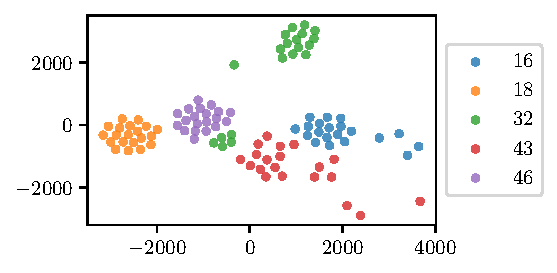
\includegraphics{./figures/data_visualization/N5R1[0]-t-SNE (metric=cosine), X_heights.pdf}
\caption{t-SNE 2-D projection of an example ``N5R1'' admixture (4, 16, 20, 20, 20), cosine distance}
\label{fig:N5R1[0]-t-SNE (metric=cosine), X_heights}
\end{figure}
\begin{figure}
\centering
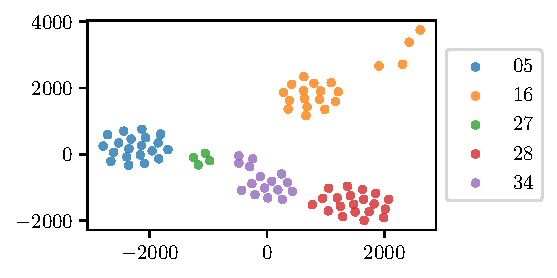
\includegraphics{./figures/data_visualization/N5R2[0]-t-SNE (metric=cosine), X_heights.pdf}
\caption{t-SNE 2-D projection of an example ``N5R2'' admixture (4, 16, 20, 20, 20), cosine distance}
\label{fig:N5R2[0]-t-SNE (metric=cosine), X_heights}
\end{figure}
\begin{figure}
\centering
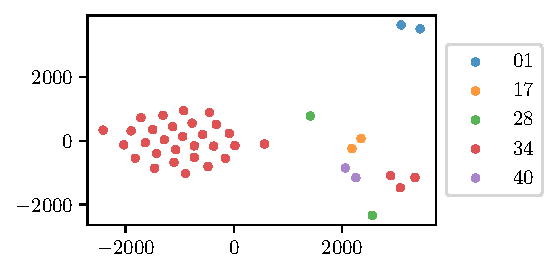
\includegraphics{./figures/data_visualization/N5R3[0]-t-SNE (metric=cosine), X_heights.pdf}
\caption{t-SNE 2-D projection of an example ``N5R3'' admixture (2, 2, 2, 2, 32), cosine distance}
\label{fig:N5R3[0]-t-SNE (metric=cosine), X_heights}
\end{figure}

In comparison, the example data visualization in Figures \ref{fig:N5R1[0]-PCA, X_heights_normalized_log}, \ref{fig:N5R2[0]-PCA, X_heights_normalized_log}, and \ref{fig:N5R3[0]-PCA, X_heights_normalized_log} show results using PCA on logarithm of normalized EPG data. It is apparent that PCA does not clearly separate some EPGs of genotypes 32 and 43 in the example ``N5R1'' admixture; nor genotypes 26 and 34 in the example ``N5R2'' admixture; nor genotypes 17, 28, 34, and 40 in the example ``N5R3'' admixture.

Overall, these examples show that although data visualization of EPG data could be helpful in providing a sense of how the data are structured, it easily provides false results given noisy EPGs.

\begin{figure}
\centering
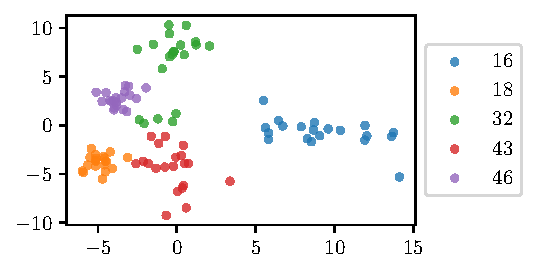
\includegraphics{./figures/data_visualization/N5R1[0]-PCA, X_heights_normalized_log.pdf}
\caption{PCA 2-D projection of an example ``N5R1'' admixture (4, 16, 20, 20, 20)}
\label{fig:N5R1[0]-PCA, X_heights_normalized_log}
\end{figure}
\begin{figure}
\centering
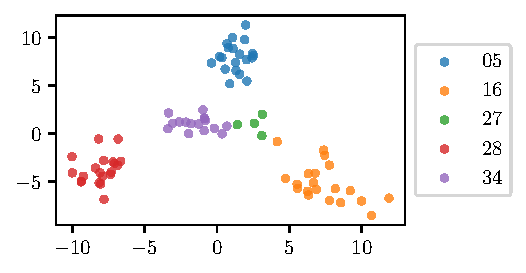
\includegraphics{./figures/data_visualization/N5R2[0]-PCA, X_heights_normalized_log.pdf}
\caption{PCA 2-D projection of an example ``N5R2'' admixture (4, 16, 20, 20, 20)}
\label{fig:N5R2[0]-PCA, X_heights_normalized_log}
\end{figure}
\begin{figure}
\centering
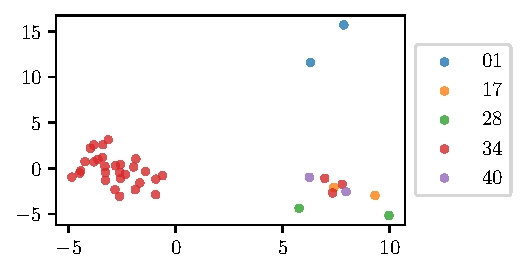
\includegraphics{./figures/data_visualization/N5R3[0]-PCA, X_heights_normalized_log.pdf}
\caption{PCA 2-D projection of an example ``N5R3'' admixture (2, 2, 2, 2, 32)}
\label{fig:N5R3[0]-PCA, X_heights_normalized_log}
\end{figure}

\section{Summary}

Although not the main subject of this thesis, the preparatory work is a prerequisite to the follow-on work in the remainder of this thesis. We have described the several preparatory tasks, for which independent development of software has been done. We have described their connections to their counterparts in \cite{odonnell_clustering_2021}. We have given examples of how noisy EPG data present problems for data visualization and clustering.
